\section{超分实验}

\subsection{MetaSR}
\begin{frame}{当前章节}
    \tableofcontents[currentsection, currentsubsection]
\end{frame}

\begin{frame}{MetaSR} 
    先前绝大多数深度学习超分方法
    \begin{itemize}
        \item 缩放系数与模型独立
        \item 只考虑若干缩放系数且必须为整数
    \end{itemize}

    Meta-SR首次通过单一模型解决了超分辨率的任意缩放因子问题(包括非整数因子), 用提出的Meta-Upscale模块代替传统上采样模块, 以下为模块三部分:
    
    \begin{itemize}
        \item Location Projection
        \item Weight Prediction
        \item Feature Mapping
    \end{itemize}
    
\end{frame}

\subsection{MetaSR初步结果}

\begin{frame}{当前章节}
    \tableofcontents[currentsection, currentsubsection]
\end{frame}

\begin{frame}{MetaSR初步结果}
    \begin{figure}[!htbp]
        \centering
        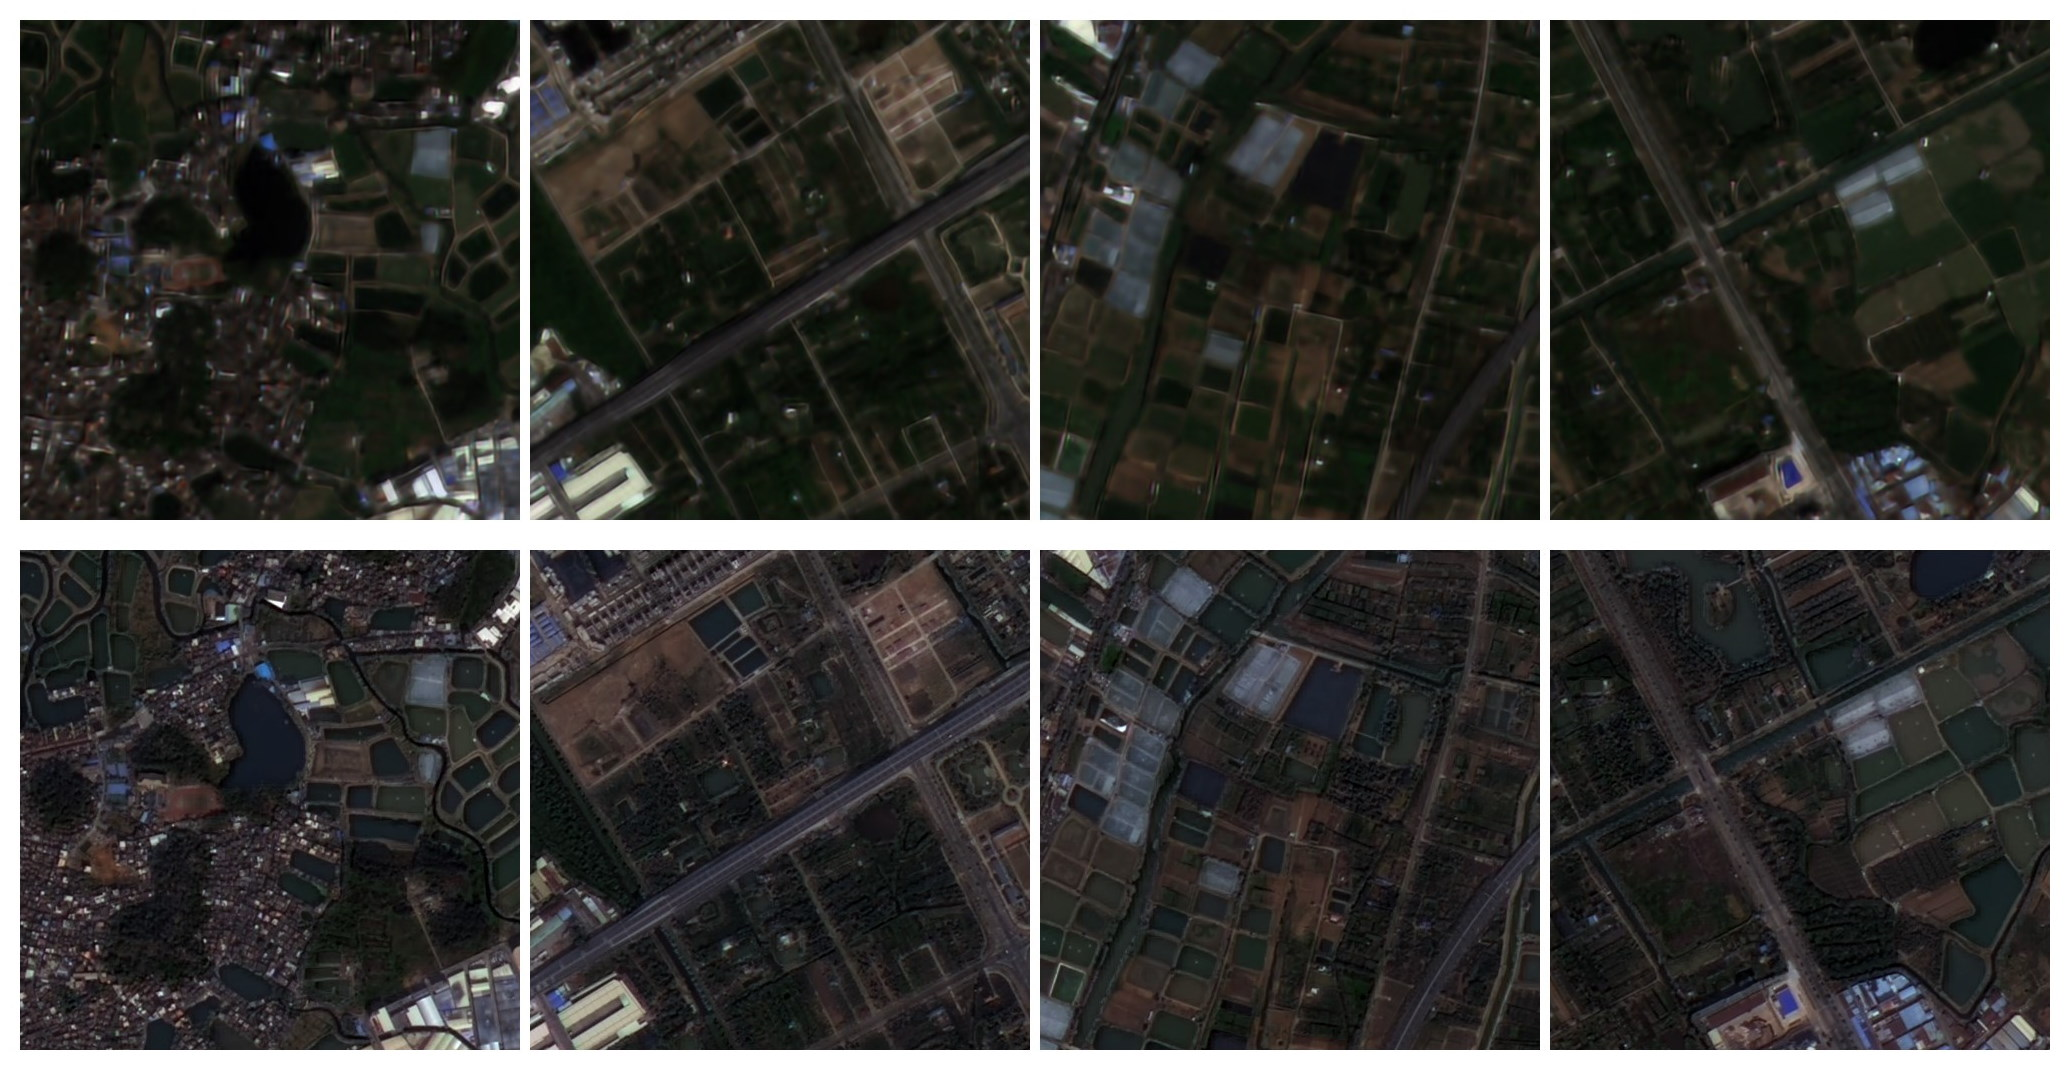
\includegraphics[width=0.9\textwidth]{pic/chap0101.jpg}
        \label{fig:0101}
        \caption{MetaSR结果\\从上至下依次为metaSR, GroudTruth}        
    \end{figure}  
\end{frame}